%% Nothing to modify here.
%% make sure to include this before anything else

\documentclass[10pt]{beamer}
\usetheme{Szeged}

% packages
\usepackage{color}
\usepackage{listings}

% color definitions
\definecolor{mygreen}{rgb}{0,0.6,0}
\definecolor{mygray}{rgb}{0.5,0.5,0.5}
\definecolor{mymauve}{rgb}{0.58,0,0.82}

% re-format the title frame page
\makeatletter
\def\supertitle#1{\gdef\@supertitle{#1}}%
\setbeamertemplate{title page}
{
  \vbox{}
  \vfill
  \begin{centering}
  \begin{beamercolorbox}[sep=8pt,center]{title}
      \usebeamerfont{supertitle}\@supertitle
   \end{beamercolorbox}
    \begin{beamercolorbox}[sep=8pt,center]{title}
      \usebeamerfont{title}\inserttitle\par%
      \ifx\insertsubtitle\@empty%
      \else%
        \vskip0.25em%
        {\usebeamerfont{subtitle}\usebeamercolor[fg]{subtitle}\insertsubtitle\par}%
      \fi%     
    \end{beamercolorbox}%
    \vskip1em\par
    \begin{beamercolorbox}[sep=8pt,center]{author}
      \usebeamerfont{author}\insertauthor
    \end{beamercolorbox}
    \begin{beamercolorbox}[sep=8pt,center]{institute}
      \usebeamerfont{institute}\insertinstitute
    \end{beamercolorbox}
    \begin{beamercolorbox}[sep=8pt,center]{date}
      \usebeamerfont{date}\insertdate
    \end{beamercolorbox}\vskip0.5em
    {\usebeamercolor[fg]{titlegraphic}\inserttitlegraphic\par}
  \end{centering}
  \vfill
}
\makeatother

% insert frame number
\expandafter\def\expandafter\insertshorttitle\expandafter{%
      \insertshorttitle\hfill%
\insertframenumber\,/\,\inserttotalframenumber}

% preset-listing options
\lstset{
  backgroundcolor=\color{white},   
  % choose the background color; 
  % you must add \usepackage{color} or \usepackage{xcolor}
  basicstyle=\footnotesize,        
  % the size of the fonts that are used for the code
  breakatwhitespace=false,         
  % sets if automatic breaks should only happen at whitespace
  breaklines=true,                 % sets automatic line breaking
  captionpos=b,                    % sets the caption-position to bottom
  commentstyle=\color{mygreen},    % comment style
  % deletekeywords={...},            
  % if you want to delete keywords from the given language
  extendedchars=true,              
  % lets you use non-ASCII characters; 
  % for 8-bits encodings only, does not work with UTF-8
  frame=single,                    % adds a frame around the code
  keepspaces=true,                 
  % keeps spaces in text, 
  % useful for keeping indentation of code 
  % (possibly needs columns=flexible)
  keywordstyle=\color{blue},       % keyword style
  % morekeywords={*,...},            
  % if you want to add more keywords to the set
  numbers=left,                    
  % where to put the line-numbers; possible values are (none, left, right)
  numbersep=5pt,                   
  % how far the line-numbers are from the code
  numberstyle=\tiny\color{mygray}, 
  % the style that is used for the line-numbers
  rulecolor=\color{black},         
  % if not set, the frame-color may be changed on line-breaks 
  % within not-black text (e.g. comments (green here))
  stepnumber=1,                    
  % the step between two line-numbers. 
  % If it's 1, each line will be numbered
  stringstyle=\color{mymauve},     % string literal style
  tabsize=4,                       % sets default tabsize to 4 spaces
  title=\lstname                   
  % show the filename of files included with \lstinputlisting; 
  % also try caption instead of title
}

% macro for code inclusion
\newcommand{\includecode}[2][c]{
	\lstinputlisting[caption=#2, style=custom#1]{#2}
}	% nothing to do here
%% Fill in metadata here that do not change over the course
%% They all are marked with the term "TODO". 
%% Search functions usually do the trick

% TODO select the targeted language
\usepackage[english]{babel}
% \usepackage[ngerman]{babel}

% TODO select the encoding
\usepackage[utf8]{inputenc}
% usepackage[latin1]{inputenc}

\newcommand{\course}{
	% TODO replace this with the name of the course
	cadvanced
}

\author{
	% TODO fill in the authors name
	Tony Template
}

\lstset{
	% TODO adapt these settings to your mainly used language
	% also see http://en.wikibooks.org/wiki/LaTeX/Source_Code_Listings
	% NOTE you can override these settings in individual cases 
	language = C,
	showspaces = false,
	showtabs = false,
	showstringspaces = false,
	escapechar = @
} % TODO modify this if you have not already done so

% meta-information
\newcommand{\topic}{
	Advanced data structures
}

\usepackage{tikz}

% nothing to do here
\title{\topic}
\supertitle{\course}
\date{}

% the actual document
\begin{document}

\maketitle

\begin{frame}{Contents}
	\tableofcontents
\end{frame}

\begin{frame}
	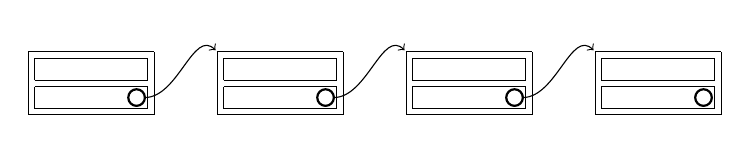
\begin{tikzpicture}[scale=.8]
		\draw (0,0) -- (0,1);
		\draw (0,0) -- (2,0);
		\draw (0,1) -- (2,1);
		\draw (2,0) -- (2,1);
		
		\draw (.1,.1) -- (.1,.45);
		\draw (.1,.1) -- (1.9,.1);
		\draw (.1,.45) -- (1.9,.45);
		\draw (1.9,.1) -- (1.9,.45);
		
		\node[circle, thick, draw=black, minimum size=6pt, inner sep = 0pt] at (1.72,.275) {};
		\draw (1.85,.275) edge[out=0,in=135,->,shorten >=.2ex] (3,1);
		
		\draw (.1,.55) -- (.1,.9);
		\draw (.1,.55) -- (1.9,.55);
		\draw (.1,.9) -- (1.9,.9);
		\draw (1.9,.55) -- (1.9,.9);
		
		
		\draw (3,0) -- (3,1);
		\draw (3,0) -- (5,0);
		\draw (3,1) -- (5,1);
		\draw (5,0) -- (5,1);
		
		\draw (3.1,.1) -- (3.1,.45);
		\draw (3.1,.1) -- (4.9,.1);
		\draw (3.1,.45) -- (4.9,.45);
		\draw (4.9,.1) -- (4.9,.45);
		\node[circle, thick, draw=black, minimum size=6pt, inner sep = 0pt] at (4.72,.275) {};
		\draw (4.85,.275) edge[out=0,in=135,->,shorten >=.2ex] (6,1);
		
		
		\draw (3.1,.55) -- (3.1,.9);
		\draw (3.1,.55) -- (4.9,.55);
		\draw (3.1,.9) -- (4.9,.9);
		\draw (4.9,.55) -- (4.9,.9);
		
		
		\draw (6,0) -- (6,1);
		\draw (6,0) -- (8,0);
		\draw (6,1) -- (8,1);
		\draw (8,0) -- (8,1);
		
		\draw (6.1,.1) -- (6.1,.45);
		\draw (6.1,.1) -- (7.9,.1);
		\draw (6.1,.45) -- (7.9,.45);
		\draw (7.9,.1) -- (7.9,.45);
		\node[circle, thick, draw=black, minimum size=6pt, inner sep = 0pt] at (7.72,.275) {};
		\draw (7.85,.275) edge[out=0,in=135,->,shorten >=.2ex] (9,1);
		
		\draw (6.1,.55) -- (6.1,.9);
		\draw (6.1,.55) -- (7.9,.55);
		\draw (6.1,.9) -- (7.9,.9);
		\draw (7.9,.55) -- (7.9,.9);
		
		
		\draw (9,0) -- (9,1);
		\draw (9,0) -- (11,0);
		\draw (9,1) -- (11,1);
		\draw (11,0) -- (11,1);
		
		\draw (9.1,.1) -- (9.1,.45);
		\draw (9.1,.1) -- (10.9,.1);
		\draw (9.1,.45) -- (10.9,.45);
		\draw (10.9,.1) -- (10.9,.45);
		\node[circle, thick, draw=black, minimum size=6pt, inner sep = 0pt] at (10.72,.275) {};
		
		\draw (9.1,.55) -- (9.1,.9);
		\draw (9.1,.55) -- (10.9,.55);
		\draw (9.1,.9) -- (10.9,.9);
		\draw (10.9,.55) -- (10.9,.9);
		
	\end{tikzpicture}
\end{frame}

% nothing to do from here on
\end{document}
